\documentclass{standalone}
\usepackage{tikz}
\usetikzlibrary{patterns, positioning}


\begin{document}
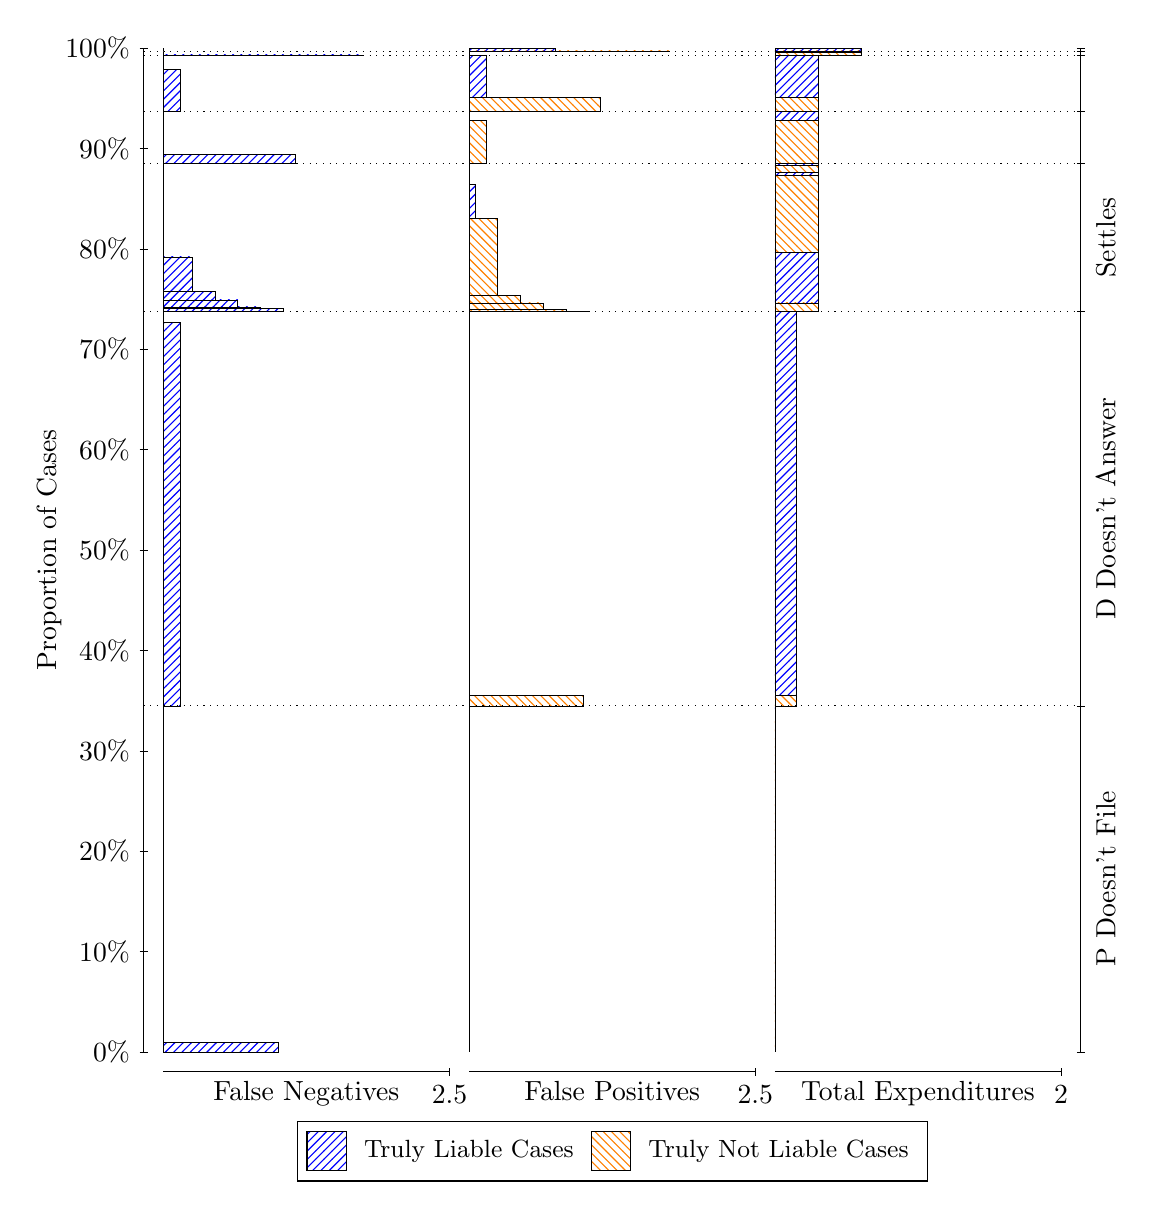
\begin{tikzpicture}
\draw[black, very thin] (1.5,1.75) -- (1.5,14.5);
\node[rotate=90, text=black, anchor=center] at (0.3, 8.125) {Proportion of Cases};
\draw[black, very thin] (1.45,1.75) -- (1.55,1.75);
\node[text=black, anchor=east] at (1.45, 1.75) {0\%};
\draw[black, very thin] (1.45,3.025) -- (1.55,3.025);
\node[text=black, anchor=east] at (1.45, 3.025) {10\%};
\draw[black, very thin] (1.45,4.3) -- (1.55,4.3);
\node[text=black, anchor=east] at (1.45, 4.3) {20\%};
\draw[black, very thin] (1.45,5.575) -- (1.55,5.575);
\node[text=black, anchor=east] at (1.45, 5.575) {30\%};
\draw[black, very thin] (1.45,6.85) -- (1.55,6.85);
\node[text=black, anchor=east] at (1.45, 6.85) {40\%};
\draw[black, very thin] (1.45,8.125) -- (1.55,8.125);
\node[text=black, anchor=east] at (1.45, 8.125) {50\%};
\draw[black, very thin] (1.45,9.4) -- (1.55,9.4);
\node[text=black, anchor=east] at (1.45, 9.4) {60\%};
\draw[black, very thin] (1.45,10.675) -- (1.55,10.675);
\node[text=black, anchor=east] at (1.45, 10.675) {70\%};
\draw[black, very thin] (1.45,11.95) -- (1.55,11.95);
\node[text=black, anchor=east] at (1.45, 11.95) {80\%};
\draw[black, very thin] (1.45,13.225) -- (1.55,13.225);
\node[text=black, anchor=east] at (1.45, 13.225) {90\%};
\draw[black, very thin] (1.45,14.5) -- (1.55,14.5);
\node[text=black, anchor=east] at (1.45, 14.5) {100\%};

\draw[black, very thin] (13.4,1.75) -- (13.4,14.5);
\draw[black, very thin] (13.35,1.75) -- (13.45,1.75);
\node[anchor=west] at (13.35, 1.75) {};
\draw[black, very thin] (13.35,6.1462) -- (13.45,6.1462);
\node[anchor=west] at (13.35, 6.1462) {};
\draw[black, very thin] (13.35,11.153) -- (13.45,11.153);
\node[anchor=west] at (13.35, 11.153) {};
\draw[black, very thin] (13.35,13.033) -- (13.45,13.033);
\node[anchor=west] at (13.35, 13.033) {};
\draw[black, very thin] (13.35,13.697) -- (13.45,13.697);
\node[anchor=west] at (13.35, 13.697) {};
\draw[black, very thin] (13.35,14.406) -- (13.45,14.406);
\node[anchor=west] at (13.35, 14.406) {};
\draw[black, very thin] (13.35,14.456) -- (13.45,14.456);
\node[anchor=west] at (13.35, 14.456) {};
\draw[black, very thin] (13.35,14.5) -- (13.45,14.5);
\node[anchor=west] at (13.35, 14.5) {};

\draw[black, very thin, pattern color=blue, pattern=north east lines] (1.75,1.75) rectangle (3.2033,1.8672);
\draw[black, very thin, pattern color=orange, pattern=north west lines] (1.75,1.8672) rectangle (1.75,6.1462);
\draw[black, very thin, pattern color=blue, pattern=north east lines] (1.75,6.1462) rectangle (1.968,11.018);
\draw[black, very thin, pattern color=orange, pattern=north west lines] (1.75,11.018) rectangle (1.75,11.153);
\draw[black, very thin, pattern color=blue, pattern=north east lines] (1.75,11.153) rectangle (3.276,11.19);
\draw[black, very thin, pattern color=blue, pattern=north east lines] (1.75,11.19) rectangle (2.9853,11.212);
\draw[black, very thin, pattern color=blue, pattern=north east lines] (1.75,11.212) rectangle (2.6947,11.301);
\draw[black, very thin, pattern color=blue, pattern=north east lines] (1.75,11.301) rectangle (2.404,11.413);
\draw[black, very thin, pattern color=blue, pattern=north east lines] (1.75,11.413) rectangle (2.1133,11.848);
\draw[black, very thin, pattern color=orange, pattern=north west lines] (1.75,11.848) rectangle (1.75,13.033);
\draw[black, very thin, pattern color=blue, pattern=north east lines] (1.75,13.033) rectangle (3.4213,13.151);
\draw[black, very thin, pattern color=orange, pattern=north west lines] (1.75,13.151) rectangle (1.75,13.697);
\draw[black, very thin, pattern color=blue, pattern=north east lines] (1.75,13.697) rectangle (1.968,14.227);
\draw[black, very thin, pattern color=orange, pattern=north west lines] (1.75,14.227) rectangle (1.75,14.406);
\draw[black, very thin, pattern color=blue, pattern=north east lines] (1.75,14.406) rectangle (4.2933,14.413);
\draw[black, very thin, pattern color=orange, pattern=north west lines] (1.75,14.413) rectangle (1.75,14.456);
\draw[black, very thin, pattern color=orange, pattern=north west lines] (1.75,14.456) rectangle (1.75,14.464);
\draw[black, very thin, pattern color=blue, pattern=north east lines] (1.75,14.464) rectangle (1.75,14.5);
\draw[black, very thin, pattern color=orange, pattern=north west lines] (5.6333,1.75) rectangle (5.6333,6.029);
\draw[black, very thin, pattern color=blue, pattern=north east lines] (5.6333,6.029) rectangle (5.6333,6.1462);
\draw[black, very thin, pattern color=orange, pattern=north west lines] (5.6333,6.1462) rectangle (7.0867,6.2812);
\draw[black, very thin, pattern color=blue, pattern=north east lines] (5.6333,6.2812) rectangle (5.6333,11.153);
\draw[black, very thin, pattern color=orange, pattern=north west lines] (5.6333,11.153) rectangle (7.1593,11.16);
\draw[black, very thin, pattern color=orange, pattern=north west lines] (5.6333,11.16) rectangle (6.8687,11.182);
\draw[black, very thin, pattern color=orange, pattern=north west lines] (5.6333,11.182) rectangle (6.578,11.264);
\draw[black, very thin, pattern color=orange, pattern=north west lines] (5.6333,11.264) rectangle (6.2873,11.356);
\draw[black, very thin, pattern color=orange, pattern=north west lines] (5.6333,11.356) rectangle (5.9967,12.338);
\draw[black, very thin, pattern color=blue, pattern=north east lines] (5.6333,12.338) rectangle (5.706,12.773);
\draw[black, very thin, pattern color=blue, pattern=north east lines] (5.6333,12.773) rectangle (5.6333,13.033);
\draw[black, very thin, pattern color=orange, pattern=north west lines] (5.6333,13.033) rectangle (5.8513,13.579);
\draw[black, very thin, pattern color=blue, pattern=north east lines] (5.6333,13.579) rectangle (5.6333,13.697);
\draw[black, very thin, pattern color=orange, pattern=north west lines] (5.6333,13.697) rectangle (7.3047,13.876);
\draw[black, very thin, pattern color=blue, pattern=north east lines] (5.6333,13.876) rectangle (5.8513,14.406);
\draw[black, very thin, pattern color=orange, pattern=north west lines] (5.6333,14.406) rectangle (5.6333,14.45);
\draw[black, very thin, pattern color=blue, pattern=north east lines] (5.6333,14.45) rectangle (5.6333,14.456);
\draw[black, very thin, pattern color=orange, pattern=north west lines] (5.6333,14.456) rectangle (8.1767,14.464);
\draw[black, very thin, pattern color=blue, pattern=north east lines] (5.6333,14.464) rectangle (6.7233,14.5);
\draw[black, very thin, pattern color=orange, pattern=north west lines] (9.5167,1.75) rectangle (9.5167,6.029);
\draw[black, very thin, pattern color=blue, pattern=north east lines] (9.5167,6.029) rectangle (9.5167,6.1462);
\draw[black, very thin, pattern color=orange, pattern=north west lines] (9.5167,6.1462) rectangle (9.7892,6.2812);
\draw[black, very thin, pattern color=blue, pattern=north east lines] (9.5167,6.2812) rectangle (9.7892,11.153);
\draw[black, very thin, pattern color=orange, pattern=north west lines] (9.5167,11.153) rectangle (10.062,11.264);
\draw[black, very thin, pattern color=blue, pattern=north east lines] (9.5167,11.264) rectangle (10.062,11.9);
\draw[black, very thin, pattern color=orange, pattern=north west lines] (9.5167,11.9) rectangle (10.062,12.882);
\draw[black, very thin, pattern color=blue, pattern=north east lines] (9.5167,12.882) rectangle (10.062,12.918);
\draw[black, very thin, pattern color=orange, pattern=north west lines] (9.5167,12.918) rectangle (10.062,13.011);
\draw[black, very thin, pattern color=blue, pattern=north east lines] (9.5167,13.011) rectangle (10.062,13.033);
\draw[black, very thin, pattern color=orange, pattern=north west lines] (9.5167,13.033) rectangle (10.062,13.579);
\draw[black, very thin, pattern color=blue, pattern=north east lines] (9.5167,13.579) rectangle (10.062,13.697);
\draw[black, very thin, pattern color=orange, pattern=north west lines] (9.5167,13.697) rectangle (10.062,13.876);
\draw[black, very thin, pattern color=blue, pattern=north east lines] (9.5167,13.876) rectangle (10.062,14.406);
\draw[black, very thin, pattern color=orange, pattern=north west lines] (9.5167,14.406) rectangle (10.607,14.45);
\draw[black, very thin, pattern color=blue, pattern=north east lines] (9.5167,14.45) rectangle (10.607,14.456);
\draw[black, very thin, pattern color=orange, pattern=north west lines] (9.5167,14.456) rectangle (10.607,14.464);
\draw[black, very thin, pattern color=blue, pattern=north east lines] (9.5167,14.464) rectangle (10.607,14.5);
\draw[black, dotted] (1.5,6.1462) -- (13.4,6.1462);
\draw[black, dotted] (1.5,11.153) -- (13.4,11.153);
\draw[black, dotted] (1.5,13.033) -- (13.4,13.033);
\draw[black, dotted] (1.5,13.697) -- (13.4,13.697);
\draw[black, dotted] (1.5,14.406) -- (13.4,14.406);
\draw[black, dotted] (1.5,14.456) -- (13.4,14.456);
\draw[black, very thin] (1.75,1.5) -- (5.3833,1.5);
\node[text=black, anchor=north] at (3.5667, 1.5) {False Negatives};
\draw[black, very thin] (5.3833,1.45) -- (5.3833,1.55);
\node[text=black, anchor=north] at (5.3833, 1.45) {2.5};

\draw[black, very thin] (5.6333,1.5) -- (9.2667,1.5);
\node[text=black, anchor=north] at (7.45, 1.5) {False Positives};
\draw[black, very thin] (9.2667,1.45) -- (9.2667,1.55);
\node[text=black, anchor=north] at (9.2667, 1.45) {2.5};

\draw[black, very thin] (9.5167,1.5) -- (13.15,1.5);
\node[text=black, anchor=north] at (11.333, 1.5) {Total Expenditures};
\draw[black, very thin] (13.15,1.45) -- (13.15,1.55);
\node[text=black, anchor=north] at (13.15, 1.45) {2};

\node[text=black, centered, rotate=90] at (13.72, 3.9481) {P Doesn't File};
\node[text=black, centered, rotate=90] at (13.72, 8.6498) {D Doesn't Answer};
\node[text=black, centered, rotate=90] at (13.72, 12.093) {Settles};





\draw (7.449999999999999,1.5) node[draw=none] (baseCoordinate) {};
\begin{scope}[align=center]
        \matrix[scale=0.5, draw=black, below=0.5cm of baseCoordinate, nodes={draw}, column sep=0.1cm]{
            \node[rectangle, draw, minimum width=0.5cm, minimum height=0.5cm, pattern color=blue, pattern=north east lines] {}; &
            \node[draw=none, font=\small, text=black] (B) {Truly Liable Cases}; &
            \node[rectangle, draw, minimum width=0.5cm, minimum height=0.5cm, pattern color=orange, pattern=north west lines] {}; &
            \node[draw=none, font=\small, text=black] (B) {Truly Not Liable Cases}; \\
            };
\end{scope}

\end{tikzpicture}
\end{document}